\begin{pastexam}[label={px:nchu-113-dsa-24}]{中興資工所甲組 113 學年度 申論題 PART 1 第 6 題}
（問答）

(6\%) Use Prim's algorithm starting at node A to compute the Minimum Spanning Tree (MST) of the graph shown
right. Please report the edges of the MST in the order in which Prim's algorithm adds them to the MST. Use
the format [node1, node2] to denote the edge connected by node1 and node 2; for example, [A, B] indicates
the edge connected by the node A and the node B.
\begin{center}
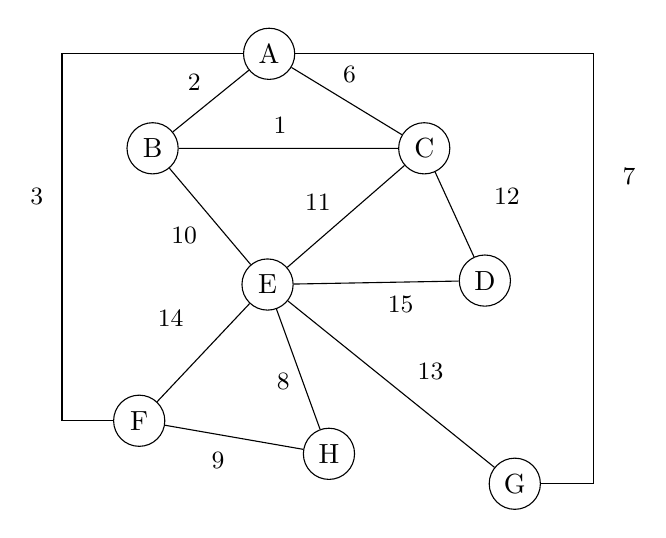
\begin{tikzpicture}[v/.style={circle,draw,minimum size=6.5mm,inner sep=1pt},lab/.style={font=\small,inner sep=1pt}]
\node[v] (A) at (3.28,5.46) {A};
\node[v] (B) at (1.80,4.26) {B};
\node[v] (C) at (5.25,4.26) {C};
\node[v] (E) at (3.26,2.53) {E};
\node[v] (D) at (6.02,2.58) {D};
\node[v] (F) at (1.63,0.80) {F};
\node[v] (H) at (4.04,0.38) {H};
\node[v] (G) at (6.40,0) {G};
\draw (A) -- (B) (A) -- (C) (B) -- (C) (B) -- (E) (C) -- (E) (C) -- (D)
  (E) -- (D) (E) -- (F) (E) -- (H) (E) -- (G) (F) -- (H);
\draw (A.west) -- (0.65,5.46) -- (0.65,0.80) -- (F.west);
\draw (A.east) -- (7.40,5.46) -- (7.40,0) -- (G.east);
\node[lab] at (2.33,5.10) {2};
\node[lab] at (4.30,5.20) {6};
\node[lab] at (3.42,4.55) {1};
\node[lab] at (2.20,3.15) {10};
\node[lab] at (3.90,3.57) {11};
\node[lab] at (6.30,3.65) {12};
\node[lab] at (4.95,2.28) {15};
\node[lab] at (2.03,2.10) {14};
\node[lab] at (3.46,1.30) {8};
\node[lab] at (5.33,1.43) {13};
\node[lab] at (2.63,0.30) {9};
\node[lab] at (0.33,3.65) {3};
\node[lab] at (7.85,3.90) {7};
\end{tikzpicture}
\end{center}
\end{pastexam}

\begin{pastsoln}
答案：[A, B]、[B, C]、[A, F]、[A, G]、[F, H]、[H, E]、[C, D]，總權重 $42$。

圖上的邊（外框那兩條是 $A$--$F$ 和 $A$--$G$）：
$AB = 2$、$AF = 3$、$AC = 6$、$AG = 7$、$BC = 1$、$BE = 10$、$CE = 11$、$CD = 12$、$ED = 15$、$EF = 14$、
$EH = 8$、$EG = 13$、$FH = 9$。 所有權重都不同，MST 唯一，Prim 每一步的選擇也唯一。

Prim 從 $A$ 開始，每一步加入「一端在樹裡、一端不在」的邊中權重最小的（資結書第~24.3~節）：
\begin{center}
\small
\begin{tabular}{clll}
\toprule
步 & 樹裡的頂點 & 跨出去的候選邊 & 加入 \\
\midrule
1 & $A$ & $AB\,2$、$AF\,3$、$AC\,6$、$AG\,7$ & [A, B] \\
2 & $A, B$ & $BC\,1$、$AF\,3$、$AC\,6$、$AG\,7$、$BE\,10$ & [B, C] \\
3 & $A, B, C$ & $AF\,3$、$AG\,7$、$BE\,10$、$CE\,11$、$CD\,12$ & [A, F] \\
4 & $A, B, C, F$ & $AG\,7$、$FH\,9$、$BE\,10$、$CE\,11$、$CD\,12$、$EF\,14$ & [A, G] \\
5 & $+\,G$ & $FH\,9$、$BE\,10$、$CE\,11$、$CD\,12$、$EG\,13$、$EF\,14$ & [F, H] \\
6 & $+\,H$ & $EH\,8$、$BE\,10$、$CE\,11$、$CD\,12$、$EG\,13$、$EF\,14$ & [H, E] \\
7 & $+\,E$ & $CD\,12$、$ED\,15$ & [C, D] \\
\bottomrule
\end{tabular}
\end{center}
（第 3 步起 $AC$ 兩端都在樹裡，不再是候選。） 七條邊連起八個頂點，總權重
$2 + 1 + 3 + 7 + 9 + 8 + 12 = 42$。

用 Kruskal 檢查：依權重 $1, 2, 3, 6, 7, 8, 9, \ldots$ 取邊，$BC, AB, AF$ 收；$AC = 6$ 成環，丟；$AG = 7$、$EH = 8$、
$FH = 9$ 收；$BE, CE$ 成環，丟；$CD = 12$ 收，滿七條。 邊集合相同，只是順序不同；題目要的是 Prim 的順序。
\end{pastsoln}
